\documentclass[preview]{standalone}
\begin{document}

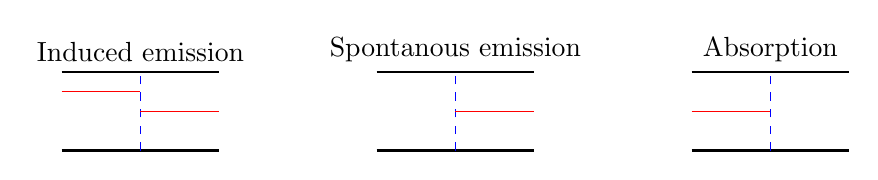
\begin{tikzpicture}[scale=1, transform shape]
% Induced Emission
\draw [thick] (2,8) -- node [above] {Induced emission} (4,8);
\draw [thick] (2,7) -- (4,7);
\draw [blue,dashed] (3,7) -- (3,8);
\draw [red] (2,7.75) -- (3,7.75);
\draw [red] (3,7.5) -- (4,7.5);

% Spontanous Emission
\draw [thick] (6,8) -- node [above] {Spontanous emission} (8,8);
\draw [thick] (6,7) -- (8,7);
\draw [blue,dashed] (7,7) -- (7,8);
\draw [red] (7,7.5) -- (8,7.5);

% Absorption
\draw [thick] (10,8) -- node [above] {Absorption} (12,8);
\draw [thick] (10,7) -- (12,7);
\draw [blue,dashed] (11,7) -- (11,8);
\draw [red] (10,7.5) -- (11,7.5);
\end{tikzpicture}

\end{document}
